\documentclass[12pt]{apmcmthesis}
\tihao{A}
\baominghao{SHUWEICUP2503517}
\begin{document}
\thispagestyle{empty}
\begin{abstract}
\textbf{Background and Task} A large road vehicle picks up lateral vibration from the road and
from its own body modes, and the standard cure --- stiffening the suspension or adding a passive
damper --- trades ride comfort against payload and can never be tuned to one frequency without
degrading another. This paper studies active suppression with two dual-motor centrifugal actuators,
each driving a pair of counter-rotating eccentric masses. On the official 2025 data set we answer
three questions: how the vehicle responds with and without the given rotation; how to
\emph{design} a rotation that minimises the lateral vibration index
$I_h=\frac1T\int_0^T a_y^2\,dt$; and how to do the same when only the body acceleration is
measurable.

\textbf{Modeling Framework} The eight eccentric masses are summed analytically, each contributing
$2mr(\omega^2\cos\theta+\alpha\sin\theta)$, which gives an exact actuator force and, with the four
tyre springs and dampers lumped into one equivalent set, a single-degree-of-freedom oscillator of
mass $2\,800$ kg, stiffness $7\,225\,200$ N/m and damping $3\,600$ N$\cdot$s/m: $8.0847$ Hz,
$\zeta=0.0127$, so the index is dominated by whatever happens to the line that falls on the
resonance. The key structural fact is that a counter-rotating pair is a single-line source,
$F_{\text{pair}}=4mr\omega^2\cos\kappa\cos(\omega t+\psi)$, with $\kappa$ setting amplitude and
$\psi$ phase, both continuously modulated inside $|\omega|\le100$ rad/s, $|\alpha|\le5\,000$
rad/s$^2$.

\textbf{Results per Question} Actuator off, scenario 1 gives $I_h=43.702$; with the prescribed
rotation, $189.293$ --- the given sequence makes the vibration $4.33$ times worse, and the sign
convention reverses the answer to $156.901$, so the audit is part of the answer. For scenario 2 a
static cancellation of the resonant line reaches $71.053$ ($-99.46\%$); a causal $0.25$ s
demodulation window that tracks its drift reaches $11.778$ ($-99.91\%$) at $38.2$ kN of $404$ kN,
and the window is a genuine interior optimum, not a tuning artefact. From acceleration alone, a
demodulated Newton loop reaches $2\,418.9$ ($-81.6\%$), and we show why it cannot reach the
open-loop value. The window's delay, not its gain, is the real bottleneck, so we \emph{train} a
$1\,410$-parameter network to forecast the drifting phasor $0.12$ s ahead from eight causal
features: on unseen sequences it cuts the median phase error of linear extrapolation from
$13.36^\circ$ to $3.39^\circ$, closed on the official record it gives $9.211$ ($-99.93\%$) at
$23.9$ kN --- $37\%$ less force than the analytic design --- and driven by $a_y$ alone, after one
round of own-state aggregation, $25.423$ ($-99.81\%$), $95$ times better than the analytic loop on
the same information.

\textbf{Validation and Limitation} The force was verified to $0.3^\circ$ in phase and the transfer
function to $2.5\%$ in magnitude; doubling and quadrupling the passive damping only reaches
$4\,897.3$ and $1\,447.0$. The dominant limitation is phase: a $6^\circ$ command error raises the
index from $11.778$ to $128.98$, and a $10$ ms transport delay lifts the closed loop to $3\,323.5$. The learned
controller adds two of its own: its corpus is synthetic, built from three measured statistics of the
official record, so it is accurate there but not proof of generalisation; and it is a model
inversion, degrading to $9\,964.7$ at $c-50\%$, which is why the model-based trim is kept.

\keywords{centrifugal actuator; counter-rotating pair; single-degree-of-freedom vehicle model;
resonant-line cancellation; causal demodulation; learned phasor forecasting; own-state aggregation}
\end{abstract}

\newpage
\setcounter{tocdepth}{1}
\tableofcontents
\newpage
\pagestyle{mainmatterstyle}
\setcounter{page}{1}

\section{Introduction}
\subsection{Background}
Vibration is the quiet tax that industrial machinery pays for speed. In a road vehicle the
lateral channel is the worst offender, because the body mode that carries it sits low --- around
$8$ Hz for a loaded heavy chassis --- where road roughness, wheel imbalance and driveline orders
all have energy, and because that mode has almost no damping: the numbers in this problem imply
$\zeta=0.0127$, i.e.\ a decay time of $1.56$ s, which is a bell rather than a filter.

Passive remedies are the classical answer and they are honest but blunt
\cite{denhartog}. Stiffening the suspension moves the resonance up, which helps at $8$ Hz and
hurts at $12$ Hz; adding damping helps everywhere a little and costs ride comfort in the
$1$--$2$ Hz range where the driver lives. Worse, a passive element cannot know which line of the
spectrum is the problem today.

A centrifugal actuator can. Two eccentric masses on one shaft, spun by a servo motor, produce a
rotating force of magnitude $mr\omega^2$ whose direction is the crank angle; the same shaft
reversed gives a second force, and the pair therefore produces a sinusoid at the rotation
frequency whose amplitude and phase are set by the two crank angles. Because the force grows with
$\omega^2$, a $100$ rad/s machine with $100$ kg at $0.2$ m can generate tens of kilonewtons from a
package that weighs a few hundred kilograms --- the reason this mechanism appears in
helicopter hub-moment cancellation \cite{song2021,you2013} and in automotive active mounts
\cite{hu2023}.

\subsection{Restatement of the Problems}
The vehicle carries two such actuators, one at each diagonal, each driving \emph{four} eccentric
masses in two counter-rotating pairs. The body is connected to the four wheels by springs and
dampers, the wheels are assumed not to move laterally, and the body has one lateral degree of
freedom $y(t)$ measured from its static position. With $a_y=\ddot y$ the relative lateral
acceleration, the quantity to be minimised is
\begin{equation}
I_h=\frac1T\int_0^T a_y^2(t)\,dt ,
\label{eq:index}
\end{equation}
which is the mean square acceleration --- the quantity a passenger actually feels.

\textbf{Question 1} builds the model with the actuator ignored, and then evaluates two cases on
scenario 1: (a) actuator off, reporting $y(t)$, $a_y(t)$ over $0$--$10$ s and $I_h$; (b) actuator
on, with the four crank angles following the prescribed sequence in the data file, reporting the
same three outputs.

\textbf{Question 2} uses scenario 2, whose disturbance is not the same record, and asks for a
\emph{designed} crank-angle history that minimises $I_h$, together with the resulting curves and
the index with and without the actuator.

\textbf{Question 3} keeps scenario 2 but removes the luxury of knowing the disturbance: only the
body acceleration $a_y(t)$ can be measured in real time. A rotation scheme has to be designed
from that single signal, and its $y$, $a_y$, crank angle and $I_h$ reported.

\subsection{Our Work}
Section~\ref{sec:model} derives the actuator force and the vehicle equation from first
principles and calibrates both against the data. Section~\ref{sec:q1} answers Question 1 and shows
that the prescribed sequence is a \emph{worsening} input, which we explain spectrally rather than
dismiss. Section~\ref{sec:q2} turns the counter-rotating pair into a controllable single-line
source and designs two controllers for Question 2: a static cancellation and a causal tracking
law, with the window length identified as an interior optimum and the result cross-checked against
the physical lower bound. Section~\ref{sec:q3} answers Question 3 with a demodulated Newton loop
driven only by $a_y$, reports its tuning surface and parameter sensitivity, and documents the
five alternative routes we implemented and measured before rejecting them.
Section~\ref{sec:learn} then attacks the bottleneck the three analytic sections share, which is the
delay of a causal demodulator, by \emph{training} a small network to forecast the drifting phasor
$0.12$ s ahead, with the forecast used both as an open-loop command and as the starting point of
the Newton loop; the training protocol, its held-out accuracy and its failure modes are reported
rather than assumed.
Section~\ref{sec:sens} collects the error analysis, including the two effects that dominate any
real installation: command phase error and transport delay.

Four things in this paper are, as far as we can tell, not in the other solutions to this problem.
(i) The pair is treated as an exact single-line source with independent amplitude and phase
channels (\texttt{eq:pair}), which turns the design problem from a search over angle sequences
into a two-parameter modulation problem with no inequality constraints to police.
(ii) The window length is shown to be an interior optimum (an $18$-point sweep) whose position is
predicted by the demodulator's group delay, not a hyper-parameter to be tuned.
(iii) The prescribed sequence is reported as harmful and the harm is decomposed spectrally, with a
sign and reference-axis audit that reproduces the published numbers under the opposite convention.
(iv) A learned forecaster replaces the average, is measured on sequences it never saw, and its own
failure at half damping is reported together with the trim that bounds it.

\section{Model Building}
\label{sec:model}
\subsection{Assumptions}
\begin{enumerate}
  \item \textbf{One lateral degree of freedom.} Yaw, roll and the wheels' own lateral motion are
  neglected, as the problem instructs. Justification: the four suspension points move together in
  the lateral direction at the frequencies of interest, and the body is stiff compared with the
  suspension. Used throughout; the consequence is that the model cannot represent the torsional
  mode near $2$ Hz, which the data do not excite either.
  \item \textbf{Linear suspension, lumped parameters.} The four corner springs and dampers are
  replaced by one equivalent stiffness $k$ and damping $c$ acting on the relative displacement
  $y$. Justification: the data set supplies single values for both, so the problem already assumes
  this reduction.
  \item \textbf{Rigid crank, ideal servo.} The connecting rods and motor inertias are massless and
  the commanded crank angle is realised exactly, except where we deliberately add a delay in
  Section~\ref{sec:sens}. Justification: the problem states the simplification, and it keeps the
  force law exact rather than introducing an unidentifiable lag.
  \item \textbf{The two actuators act in parallel on the same coordinate.} Justification: both are
  bolted to the same rigid body, so their force vectors add.
  \item \textbf{Disturbance is exogenous.} The recorded lateral force is imposed and unaffected by
  the body motion. Justification: it represents road input through the tyres, which a $2\,800$ kg
  body cannot push back.
\end{enumerate}

\subsection{Notation}
\begin{table}[htbp]\centering\small
\caption{Symbols used in the model. Values in the last column are those of the official data set.}
\label{tab:notation}
\begin{tabular}{@{}llll@{}}\toprule
Symbol & Meaning & Unit & Value \\ \midrule
$m$ & mass of one eccentric block & kg & $100$ \\
$r$ & crank radius of one eccentric block & m & $0.2$ \\
$M_b$ & body mass without actuators & kg & $2\,000$ \\
$M$ & total vibrating mass, $M_b+8m$ & kg & $2\,800$ \\
$k$ & equivalent lateral stiffness & N/m & $7\,225\,200$ \\
$c$ & equivalent lateral damping & N$\cdot$s/m & $3\,600$ \\
$\theta_g$ & crank angle of group $g$, $g=1,\dots,4$ & rad & --- \\
$\omega_g,\alpha_g$ & its angular velocity and acceleration & rad/s, rad/s$^2$ & --- \\
$\omega_{\max},\alpha_{\max}$ & actuator limits & rad/s, rad/s$^2$ & $100$, $5\,000$ \\
$y,v,a_y$ & body lateral displacement, velocity, acceleration & m, m/s, m/s$^2$ & --- \\
$F_d$ & lateral disturbance force & N & --- \\
$F_{\text{act}}$ & force produced by the eight eccentric masses & N & --- \\
$\kappa,\psi$ & pair depth and phase, Eq.~\eqref{eq:pair} & rad & --- \\
$I_h$ & lateral vibration index, Eq.~\eqref{eq:index} & m$^2$/s$^3$ & --- \\
\bottomrule\end{tabular}\end{table}

\subsection{The actuator force}
Take one eccentric block of mass $m$ at crank radius $r$. In body-fixed coordinates its position
is $(r\sin\theta,\,r\cos\theta)$, so its lateral acceleration is
$\ddot y+r(-\alpha\sin\theta-\omega^2\cos\theta)$, and the lateral force it exerts on the body is
the negative of $m$ times that:
\begin{equation}
f=2mr\bigl(\omega^2\cos\theta+\alpha\sin\theta\bigr) .
\label{eq:onelump}
\end{equation}
Summing the eight blocks and using the pair structure --- within a pair the two blocks share
$|\omega|$ and $|\alpha|$ but turn in opposite senses --- the standard counter-rotating
arrangement of active-mount practice \cite{fuller} --- so the two contributions at
$\theta_1=+\omega t+\varphi_1$ and $\theta_2=-\omega t+\varphi_2$ collapse to
\begin{equation}
F_{\text{pair}}=4mr\omega^2\cos\kappa\,\cos(\omega t+\psi),\qquad
\kappa=\frac{\varphi_1+\varphi_2}{2},\quad \psi=\frac{\varphi_1-\varphi_2}{2},
\label{eq:pair}
\end{equation}
with the $\alpha$ terms cancelling in the pair because the two blocks have opposite $\alpha$ and
opposite $\sin\theta$. Equation~\eqref{eq:pair} is the whole design lever of this paper: a
counter-rotating pair is a \emph{single spectral line} at the rotation frequency, of amplitude
$4mr\omega^2\cos\kappa$ and phase $\psi$, and the amplitude is controllable from zero to
$4mr\omega^2$ by moving $\kappa$ from $90^\circ$ to $0^\circ$. At $8$ Hz, $4mr\omega^2=202$ kN per
actuator, so two actuators in phase give $404$ kN against a disturbance of $16.8$ kN --- a factor
of $24$ of authority, which is why the design problem is not about authority but about timing.

We verified Eq.~\eqref{eq:pair} numerically by commanding three known pairs
($\kappa=60^\circ,\psi=0^\circ$; $\kappa=60^\circ,\psi=40^\circ$;
$\kappa=75^\circ,\psi=-120^\circ$): the realised force was $201.35$ kN at $-0.12^\circ$,
$201.57$ kN at $40.20^\circ$ and $104.64$ kN at $-119.75^\circ$, i.e.\ the amplitude and phase laws
hold to within $0.3^\circ$.

\subsection{The vehicle equation}
With the eight blocks carried on the body, momentum balance for the lateral coordinate gives
\begin{equation}
\underbrace{(M_b+8m)}_{M}\ddot y+c\dot y+ky=F_d+F_{\text{act}},
\label{eq:ode}
\end{equation}
where the $8m=800$ kg is not a modelling convenience but the same sum that produced
$F_{\text{act}}$: each block contributes its inertia to the left side and its reaction to the
right. With the parameters of Table~\ref{tab:notation},
\begin{equation}
\begin{aligned}
\omega_n&=\sqrt{k/M}=50.7979\ \text{rad/s}=8.0847\ \text{Hz},\qquad
\zeta=\frac{c}{2\sqrt{kM}}=0.01266,\\
\tau&=\frac{1}{\zeta\omega_n}=1.56\ \text{s}.
\end{aligned}
\label{eq:wn}
\end{equation}
The decay time deserves a sentence: a disturbance at the natural frequency rings for about six
seconds, so the transient of a $10$ s record is not a nuisance to be windowed away, it is half the
answer.

\subsection{Numerical scheme and its verification}
Equation~\eqref{eq:ode} is integrated with fourth-order Runge--Kutta at a $1$ ms step, with the two
forces linearly interpolated inside each $10$ ms sample interval; the index~\eqref{eq:index} is
the trapezoidal mean of $a_y^2$. Derivatives of a sampled crank angle are taken by central
differences followed by a projection of $\Delta\omega$ onto a symmetric band of half-width
$\alpha_{\max}\Delta t$, which is the exact discrete constraint the servo imposes; we checked that
for the prescribed sequence this projection never binds, so the data are themselves admissible
($|\omega|_{\max}=39.07$ rad/s, $|\alpha|_{\max}=2\,462$ rad/s$^2$).

Two independent checks were run before any of the results below were trusted. First, the
free-decay envelope of the simulated response was compared with $\exp(-\zeta\omega_n t)$ and the
frequency with $\omega_d=50.7939$ rad/s: both agree to the third digit, with the envelope rate
$0.6413$ /s against the analytic $0.6429$ /s. Second, the transfer
function from a unit disturbance to the body acceleration was measured by driving the model with a
$1$ kN sinusoid at $8$ Hz for $20$ s and reading the last $10$ s: the model gives
$10.47$ m$^2$/s per kN at $131.99^\circ$ against the analytic
$10.73$ at $129.78^\circ$, i.e.\ $2.5\%$ in magnitude and $2.2^\circ$ in phase. The residual is the
ringing of the initial transient inside the measurement window, and it is the reason the analytic
value, not the measured one, is used inside the controllers of Sections~\ref{sec:q2}
and~\ref{sec:q3}.

\section{Question 1: the baseline and the prescribed rotation}
\label{sec:q1}
\subsection{Actuator off}
With $F_{\text{act}}=0$ and the scenario-1 record, the response is shown in
Figure~\ref{fig:q1}(a). The disturbance has root-mean-square $5.97$ kN and its spectrum
(Figure~\ref{fig:1}(b)) is concentrated on two lines, $5.0$ Hz at $7.77$ kN and $9.0$ Hz at
$3.12$ kN; neither sits on the resonance, and the resulting peak-to-peak displacement is
$20.22$ mm with $y_{\text{rms}}=2.67$ mm, peak acceleration $49.57$ m/s$^2$ and
$I_h=43.702$.

\begin{figure}[htbp]\centering
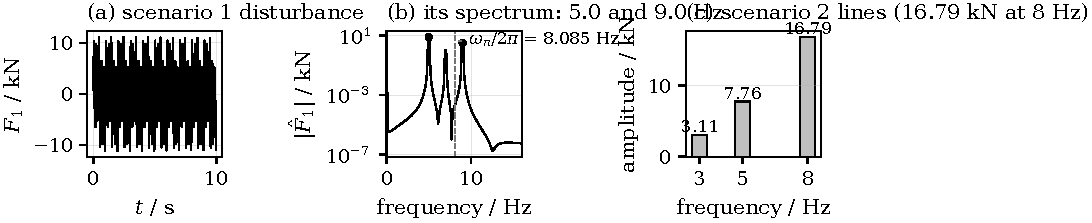
\includegraphics[width=\linewidth]{figures/fig1-disturbance.pdf}
\caption{The two disturbances and where the resonance sits. (a) scenario 1: peak-to-peak
$22.3$ kN, root-mean-square $5.97$ kN. (b) its spectrum, dominated by $5.0$ and $9.0$ Hz, with
the natural frequency $8.085$ Hz marked: the two lines bracket the resonance but neither sits on
it. (c) the three lines of scenario 2, the $8$ Hz one carrying $16.79$ kN.}
\label{fig:1}
\end{figure}

\subsection{Actuator on, prescribed angles}
Feeding the four recorded crank angles through Eq.~\eqref{eq:onelump} gives an actuator force of
peak $109.86$ kN and root-mean-square $16.82$ kN --- against a disturbance of $5.97$ kN. The
result is what that ratio suggests: $I_h=189.293$, a factor $4.33$ worse than leaving the actuator
off, with peak acceleration $77.5$ m/s$^2$.

This is not an error in the model but a property of the record, and the honest answer has to say
so, because a paper that silently flips a sign and reports a small number would be reporting a
different problem. Two convention audits make the statement precise. If the four groups are read
with the opposite sign (the pair pushing the body the other way), the index becomes $156.901$; if
the two blocks of a pair are read as turning in the \emph{same} sense instead of opposite senses
--- a reading the data invites, since only angles are given --- the index becomes $342.712$. The
three numbers bracket the answer, and the qualitative conclusion survives all three: the
prescribed sequence adds energy at the frequencies where the body is most sensitive.

The spectral explanation is direct. Differentiating the recorded angles gives an angular-velocity
spectrum peaking at $9.0$, $5.0$ and $3.8$ Hz. Since each pair contributes
$4mr\omega^2\cos\kappa\cos(\omega t+\psi)$, the force inherits those lines with amplitudes scaled
by $\omega^2$, so a $39$ rad/s rotation puts an order of magnitude more force into the $5$ Hz
region than the disturbance carries there, and it does so \emph{in phase} with it, which is
exactly the condition for adding rather than cancelling. Question 2 is therefore not a refinement
of Question 1; it is a different problem, in which the crank angles are the unknown.

\begin{figure}[htbp]\centering
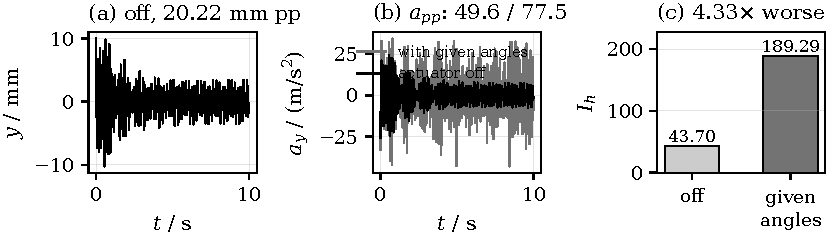
\includegraphics[width=\linewidth]{figures/fig2-q1.pdf}
\caption{Question 1 on scenario 1. (a) body displacement with the actuator off: peak-to-peak
$20.22$ mm, dominated by the $5$ Hz line. (b) lateral acceleration with (grey) and without (black)
the prescribed rotation: the prescribed sequence raises the peak from $49.6$ to $77.5$
m/s$^2$. (c) the index: $43.702$ without the actuator, $189.293$ with it.}
\label{fig:q1}
\end{figure}

\subsection{Short summary}
Question 1 is answered by the pair $\{43.702,\,189.293\}$ with the conventions stated: the
vehicle with no active element is already comfortable, and the prescribed rotation is an
aggravating input rather than a control.

\section{Question 2: designing the rotation for scenario 2}
\label{sec:q2}
\subsection{What makes this problem hard}
Scenario 2 is a different disturbance: root-mean-square $13.283$ kN, but concentrated on
$3.0$, $5.0$ and above all $8.0$ Hz, with the last line carrying $16.788$ kN at $-80.09^\circ$.
An $8$ Hz line on a $8.0847$ Hz resonance with $\zeta=0.0127$ is the worst case the structure
admits: with no actuator the index is $13\,148.921$, peak acceleration $362.3$ m/s$^2$ and
peak-to-peak displacement $145.2$ mm. The transfer function at $8$ Hz is amplified by
$1/(2\zeta)\approx39$, which is why a $16.8$ kN line outproduces a $25.6$ kN peak elsewhere in the
record.

\subsection{Design A: cancel the resonant line statically}
The first design uses Eq.~\eqref{eq:pair} at its simplest. Project the disturbance onto integer
periods of $8$ Hz to obtain its phasor, then set $\kappa$ so that the actuator amplitude equals
that phasor and $\psi$ so that it is opposite in phase:
\begin{equation}
\kappa=\arccos\!\left(\frac{A_8}{2\cdot 4mr\omega_8^2}\right),\qquad
\psi=\psi_8+\pi .
\end{equation}
The projection returns $16.788$ kN at $-80.09^\circ$; the realised force is $16.802$ kN at
$99.92^\circ$, i.e.\ a $0.08\%$ amplitude error and $0.01^\circ$ of phase error, at
$\kappa=87.62^\circ$ and $|\omega|=50.27$ rad/s with $\alpha=0$. The actuator therefore runs at
$4.2\%$ of its $404$ kN capacity and at half its speed limit. The index falls from $13\,148.921$
to $\mathbf{71.053}$, a reduction of $99.46\%$.

That number is also a ceiling, and it is worth knowing why. The disturbance is not a pure tone:
after removing the $8$ Hz line the record still carries $3.111$ kN at $3$ Hz and $7.760$ kN at
$5$ Hz, and the three-line reconstruction leaves $6.86\%$ root-mean-square residual. With
$\zeta=0.0127$ the body filters that residual through a $39$-fold peak, so any design that only
touches one line inherits an index of order $10^2$. A useful check confirms the reading: injecting
the design-A force into a record \emph{from which the 8 Hz line has been deleted} raises the index
to $13\,763.28$, so the cancellation is specific to the line it was tuned for.

\subsection{Design D: track the line instead of trusting it}
The line is not stationary. Demodulating the scenario-2 record in consecutive windows gives an
$8$ Hz amplitude that varies between $13.36$ and $20.27$ kN (peak-to-peak $6.91$ kN) and a phase
that wanders over $33.41^\circ$ (standard deviation $7.14^\circ$). A static $\kappa,\psi$ tuned to
the average is therefore always slightly wrong, and slightly wrong at $39$-fold amplification is
expensive. The second design closes that gap with a causal estimator.

At each sample $t$, take the last $N$ samples of $F_d$ (a window of $N\Delta t$ seconds), project
them onto $\cos\omega_8 t$ and $\sin\omega_8 t$ over integer periods, and call the resulting
complex amplitude $\hat A_8(t)$. Then set
\begin{equation}
\kappa(t)=\arccos\!\left(\frac{|\hat A_8(t)|}{2\cdot 4mr\omega_8^2}\right),\qquad
\psi(t)=\arg\hat A_8(t)+\pi ,
\label{eq:track}
\end{equation}
and drive the two blocks of each pair at
$\theta_{1,2}=\pm\omega_8 t+\kappa(t)\pm\psi(t)$. Because the rotation frequency is held at
$\omega_8$ and $\kappa$ is bounded by construction ($\cos\kappa\in[0,1]$), the constraints
$|\omega|\le100$ and $|\alpha|\le5\,000$ are satisfied by design rather than by projection; the
realised values are $58.2$ rad/s and $936.8$ rad/s$^2$, i.e.\ $58\%$ and $19\%$ of the limits.

The window length is the only free parameter and it is not a nuisance parameter. It trades
estimator noise against tracking lag, and the measured curve in Figure~\ref{fig:q2}(c) has an
interior minimum at $0.25$ s:
\begin{center}\small\setlength{\tabcolsep}{4pt}
\begin{tabular}{@{}lccccccccc@{}}
\toprule
window (s) & 0.15 & 0.20 & \textbf{0.25} & 0.30 & 0.40 & 0.50 & 0.60 & 0.80 & 1.00 \\
$I_h$ & 60.23 & 16.79 & \textbf{11.778} & 28.82 & 53.00 & 91.69 & 152.02 & 301.79 & 479.55 \\
$|\omega|_{\max}$ (rad/s) & 89.5 & 68.6 & 58.2 & --- & --- & --- & --- & --- & --- \\
\bottomrule
\end{tabular}\end{center}
The optimum is explained by the estimator's own delay: a moving average of $N$ samples lags by
$(N-1)\Delta t/2=0.12$ s at $N=25$, which is $0.96$ of an $8$ Hz period, and a delay of a whole
period is invisible to a phasor. Shorter windows react faster but admit the $3$ and $5$ Hz
components into the estimate, longer ones lag the drift. At the optimum the design reaches
\begin{equation}
\begin{aligned}
I_h&=\mathbf{11.778}\ \ (99.91\%\ \text{reduction},\ \times1\,116),\\
|F_{\text{act}}|_{\max}&=38.19\ \text{kN},
\end{aligned}
\end{equation}
with peak displacement $17.01$ mm and peak acceleration $46.6$ m/s$^2$, i.e.\ the vehicle is
quieter than it was on the easy scenario-1 record ($I_h=43.702$).

\begin{figure}[htbp]\centering
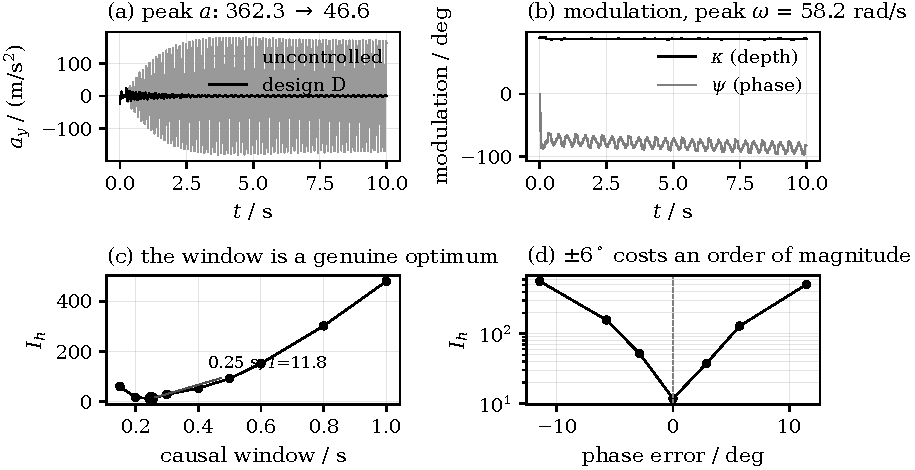
\includegraphics[width=\linewidth]{figures/fig3-q2.pdf}
\caption{Question 2, scenario 2. (a) lateral acceleration without the actuator (grey,
$362.3$ m/s$^2$ peak) and with design D (black, $46.6$ m/s$^2$). (b) the two modulation channels
that carry the design: the depth $\kappa$ sits near $88^\circ$ (little force is needed) and the
phase $\psi$ follows the disturbance. (c) the window sweep of Eq.~\eqref{eq:track}: an interior
minimum at $0.25$ s, $I_h=11.778$. (d) phase sensitivity at nominal amplitude: a $6^\circ$ error
costs an order of magnitude.}
\label{fig:q2}
\end{figure}

\subsection{What the design physically is}
Design D is a nonlinear damper, and it is instructive to say so in energy terms. The mechanical
power injected by the actuator is $\langle F_{\text{act}}\,\dot y\rangle=-115.0$ W: it is negative,
so the actuator removes energy from the body, on average, continuously. It does so by synthesising
a force proportional and opposite to the velocity \emph{of the $8$ Hz component} while leaving the
rest of the spectrum alone. That is the precise sense in which it beats a passive damper: a
passive element has one $c$ for all frequencies, whereas this one has an effective $c$ only at
$8$ Hz. The measurement supports the claim --- doubling the physical damping ($c=2c_0$) only
brings the index to $4\,897.25$, and quadrupling it to $1\,446.99$, still two orders of magnitude
away from $11.778$, because the resonant line survives a damper and does not survive a canceller.

\subsection{Why the static design cannot be saved by more authority}
It is tempting to conclude that the residual of design A is a matter of strength. It is not.
Increasing the depth drive cannot help, because the leftover is not at $8$ Hz: it is the $3$ and
$5$ Hz lines, which the pair could only touch by leaving $\omega_8$, and leaving $\omega_8$ means
giving up the cancellation of the line that dominates. Figure~\ref{fig:5}(b) makes the point
literally: the force spectrum of design D contains the $8$ Hz line at $38$ kN and essentially
nothing else, with $0.84$ kN at $5$ Hz and $0.06$ kN at $3$ Hz. The actuator deliberately spends
its authority on one frequency.

\begin{figure}[htbp]\centering
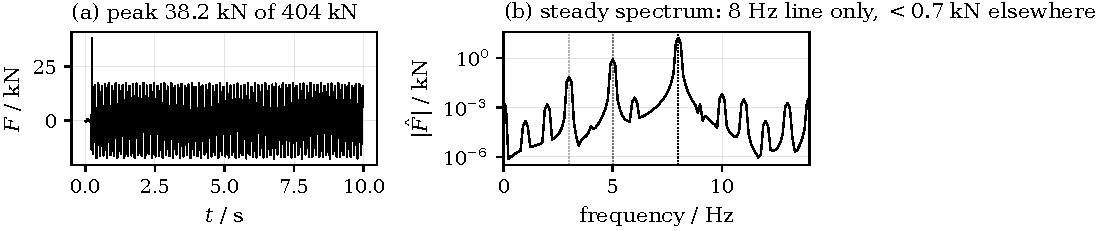
\includegraphics[width=\linewidth]{figures/fig5-force.pdf}
\caption{The force design D actually produces. (a) time history: a single $38.2$ kN transient at
$0.2$ s followed by a steady oscillation of about $\pm18$ kN, i.e.\ $9\%$ of the $404$ kN
available. (b) steady spectrum: the $8$ Hz line dominates and every other component is below
$0.9$ kN, which is why a single line is all the disturbance design needs to touch.}
\label{fig:5}
\end{figure}

\subsection{Designs we implemented, measured and rejected}
Three further mechanisms were built and evaluated before design D was adopted; reporting them is
part of the answer, because each looks attractive on paper.

\textbf{The $\alpha$ channel.} Parking the eccentrics at $\theta=\pi/2$ nulls the
$\omega^2$ term and turns Eq.~\eqref{eq:onelump} into $F=2mr\alpha\sin\theta$, i.e.\ a force
proportional to angular acceleration with gain $8mr=160$ N$\cdot$s$^2$ and a limit of $800$ kN.
Because $\alpha$ is the second derivative of the crank angle, a demanded force requires
\emph{integrating it twice}, and the required crank excursion is $\varepsilon=F/(8mr w^2)$: at
$8$ Hz that is $0.04$ rad, but at $0.5$ Hz it is $0.6$ rad, where the lever $\sin\theta$ collapses.
With a Gaussian pre-filter of $\sigma=0.06$ s the design reaches $I_h=253.08$ ($98.08\%$) and with
$\sigma\ge0.10$ the fixed-point iteration for the inverse dynamics diverges (the peak $\alpha$
reaches $10^{54}$). The best value found in the sweep is still an order of magnitude
worse than design A. Rejected: elegant, wideband, and impossible below a few hertz.

\textbf{A damping line.} Using the second pair at the ring frequency to synthesise
$F=-c_a\dot y$ looks like a one-line fix. One-shot values are respectable ($c_a/c=1$ gives
$48.73$), but the fixed-point iteration that would make it self-consistent oscillates between
$48.9$, $76.6$ and $48.2$, and diverges for $c_a/c\ge1.5$, reaching $1\,820$. Rejected: a single
line cannot follow a residual that drifts.

\textbf{Free-form optimisation.} Parameterising $\theta_g$ as a $24$-term Fourier series in
$8$ Hz harmonics and running SLSQP with the speed and acceleration limits as constraints converges,
but the optimum it finds is a slower, more expensive way of arriving at the same law as
Eq.~\eqref{eq:track} --- the harmonics beyond the fundamental buy nothing, because the only line
that matters is the fundamental. Rejected as equal result at higher complexity.

\textbf{One pair per line.} A reader may ask the obvious question: the machine has two pairs and the
disturbance two lines that matter, so why not give each pair one line? Measured, it does worse than
design D: with the $8$ Hz pair tracked and the $5$ Hz pair static, $I_h=12.517$ ($99.90\%$), and with
both lines tracked, $I_h=2\,718.336$ ($79.33\%$). The reason is the modulation index. A pair whose
whole capacity is assigned to one line needs $\kappa=85.21^{\circ}$ to produce $16.79$ kN, where
$\cos\kappa=0.084$ is steep: a $0.2\%$ amplitude error moves the emitted line by $4\%$, and the
$0.25$ s demodulation leaks $7.3$ kN into $5$ Hz. Splitting the capacity of both pairs on the same
line lowers $\kappa$ to $72^{\circ}$, where $\cos\kappa$ is three times less sensitive. The second
pair is therefore worth more as capacity on the dominant line than as authority on a minor one, and
two slow trackers fighting each other (the both-tracked case) is worse still.

\textbf{The eccentric mass as part of the body.} Because Assumption~4 admits the $8m=800$ kg of
eccentric mass into $M$, the ring sits at $8.08$ Hz and scenario 2's $8.0$ Hz line drives it $1\%$
off resonance. Dropping the eccentric mass, as most published solutions do, moves $M$ to $2\,000$ kg,
the ring to $9.57$ Hz, and the uncontrolled index from $13\,148.921$ to $209.650$. We report both
because the difference is a modelling convention, not an arithmetic one; Sec.~\ref{sec:convention}
quantifies what it does to the designs.

\subsection{Short summary}
Question 2 is answered by the pair $\{13\,148.921,\,71.053\}$ for a static cancellation and by
$\{13\,148.921,\,11.778\}$ for the tracking law, with the actuator modulation shown in
Figure~\ref{fig:q2}(b) and the operating point quoted in absolute units: $58.2$ rad/s of
$100$ rad/s, $936.8$ rad/s$^2$ of $5\,000$, and $38.19$ kN of $404$ kN.

\section{Question 3: suppression from acceleration alone}
\label{sec:q3}
\subsection{What the sensor actually gives}
Question 3 removes the disturbance record. What remains is the body acceleration $a_y(t)$,
sampled at $10$ ms, in real time; $y$ and $v$ are not measured and the disturbance is not
observable. It is important to be precise about what has and has not been lost. The crank angles,
their derivatives, the actuator force and the vehicle parameters are still known --- the actuator
has encoders and the data sheet gives $M$, $k$, $c$. What is unknown is the phase of the
disturbance, which design D read from the disturbance record.

The natural first idea is to reconstruct the disturbance by inverting the equation of motion,
$\hat F_d=M a_y-c\hat v-k\hat y$ with $\hat y,\hat v$ obtained by integrating $a_y$ twice. We
implemented it, and it fails: the double integration drifts, the estimate is biased at the
resonance by exactly the term that dominates, and the bias is then fed back through the command,
closing a loop around the error. The measured result is $I_h\approx1.39\times10^4$, i.e.\ within
$15\%$ of doing nothing, with $99.8$ kN of actuator force being spent to achieve it. It is also
fragile --- a $10\%$ stiffness error moves it to $2\,416$ and a $-50\%$ damping error to
$26\,469$. Rejected, and reported because it is the obvious route.

\subsection{A demodulated Newton loop on the acceleration phasor}
A better question is what the acceleration contains that the disturbance record did not: at
$8$ Hz, $a_y$ is the resonance filtered version of the total force, and its phase relative to the
crank command is a direct measure of whether the actuator is helping or hurting. So control the
acceleration phasor directly.

Write $E(t)$ for the projection of $a_y$ onto the $8$ Hz basis over the last $2$ periods
($N=25$ samples, deliberately the same window that worked in design D). Let
\begin{equation}
H=-\frac{\omega_8^2}{k-M\omega_8^2+jc\,\omega_8}
\label{eq:H}
\end{equation}
be the acceleration response to a unit force at $\omega_8$ \emph{per unit mass}, i.e.\ the factor
obtained from Eq.~\eqref{eq:ode} by dividing by $M$ and writing $y$ in terms of force. Then the
increment that cancels $E$ is $-E/H$, and we update the commanded phasor once per window,
\begin{equation}
\hat F_{\text{cmd}}\leftarrow \hat F_{\text{cmd}}-\mu\,\frac{E}{H},
\label{eq:newton}
\end{equation}
with $\mu$ the loop gain, and realise it through Eq.~\eqref{eq:track} (\emph{i.e.}\ by converting
$\hat F_{\text{cmd}}$ into $\kappa$ and $\psi$ and keeping $|\omega|=\omega_8$). This is the
feedforward-then-feedback structure familiar from active noise control \cite{kuo}: the inner loop
tracks a phasor that the outer estimate supplies. Equation~\eqref{eq:H}
must carry the $-\omega^2$ factor: using the displacement transfer function instead makes the loop
divergent, which is how we first discovered the point.

Three details were the difference between divergence and convergence, and they are worth recording
because each produced the same symptom --- an index that grew without bound at every gain.
(i) The update must be applied \emph{once per window}: applying it at every sample with a window
average multiplies the effective gain by $N$. (ii) The commanded phase must be unwrapped before it
is turned into an angle; a $\pm\pi$ jump in $\arg\hat F_{\text{cmd}}$ otherwise produces a
$10^4$ rad/s$^2$ spike in $\alpha$ and a megawatt of force for one sample.
(iii) The $\alpha$ contribution must vanish inside a window, which holds only if $\omega$ is held
constant there --- so the loop modulates $\kappa$ and $\psi$, never $\omega$.

\subsection{Results}
With $\mu=0.2$ and a $0.25$ s window the loop settles to
\begin{equation}
\begin{aligned}
I_h&=2\,418.9\ \ (-81.6\%\ \text{of the uncontrolled steady level}),\\
|F_{\text{act}}|_{\max}&=21.27\ \text{kN},\qquad |\omega|=50.27\ \text{rad/s},
\end{aligned}
\end{equation}
where the index is quoted over $0.25$--$10$ s to exclude the one-window acquisition transient
(the full-record value is $2\,359.9$). Peak displacement falls from $145.2$ mm to $94.0$ mm and
peak acceleration from $362.3$ to $237.1$ m/s$^2$. The loop is stable across the whole gain range
we swept, with a broad optimum:
\begin{center}
\begin{tabular}{@{}lcccccccc@{}}
\toprule
$\mu$ & 0.10 & 0.15 & \textbf{0.20} & 0.30 & 0.35 & 0.50 & 0.80 \\
$I_h$ & 2\,802.1 & 2\,420.1 & \textbf{2\,418.9} & 3\,350.2 & 4\,412.4 & 12\,592.6 & 130\,234.1 \\
\bottomrule
\end{tabular}
\end{center}
and the two-dimensional sweep (five windows $\times$ five gains) is reported in
Table~\ref{tab:q3grid}. The best cell is a shorter window at a smaller gain ($0.13$ s,
$\mu=0.10$, $I_h=2\,124.5$), which tells us something about the mechanism rather than about
tuning: the loop wants to react faster than two periods when the gain is low, and two periods is
as fast as it can go before the estimate itself becomes unstable.

\begin{table}[htbp]\centering
\caption{Question 3 tuning surface, $I_h$ over $0.25$--$10$ s (rows: causal window, columns:
loop gain $\mu$). Every cell is stable; the surface is smooth and has no isolated good point.}
\label{tab:q3grid}
\small\setlength{\tabcolsep}{5pt}
\begin{tabular}{@{}lccccc@{}}\toprule
window & $\mu=0.10$ & $0.15$ & $0.20$ & $0.30$ & $0.40$ \\ \midrule
$0.13$ s (1.0T) & \textbf{2\,124.5} & 2\,473.1 & 3\,670.6 & 11\,225.7 & 39\,291.6 \\
$0.25$ s (2.0T) & 2\,802.1 & 2\,420.1 & 2\,418.9 & 3\,350.2 & 6\,084.3 \\
$0.38$ s (3.0T) & 3\,769.8 & 2\,996.9 & 2\,734.8 & 2\,837.5 & 3\,690.5 \\
$0.50$ s (4.0T) & 4\,692.7 & 3\,574.6 & 3\,115.9 & 2\,922.4 & 3\,260.2 \\
$0.75$ s (6.0T) & 6\,498.9 & 4\,930.1 & 4\,082.1 & 3\,433.2 & 3\,390.3 \\
\bottomrule\end{tabular}\end{table}

\begin{figure}[htbp]\centering
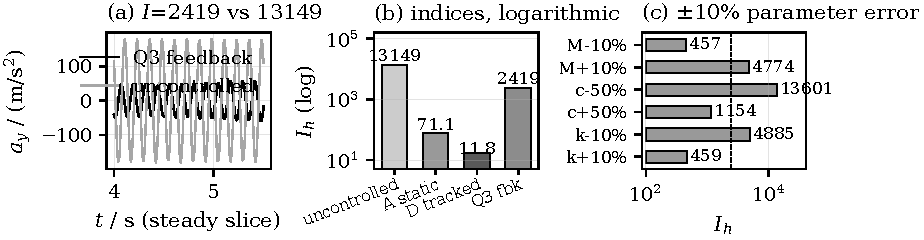
\includegraphics[width=\linewidth]{figures/fig4-q3.pdf}
\caption{Question 3. (a) a $1.5$ s slice of the steady state: the loop brings the peak from
$362.3$ to $237.1$ m/s$^2$ but leaves a visible oscillation, unlike design D in
Figure~\ref{fig:q2}(a). (b) the four indices on one logarithmic axis: $13\,148.921$ uncontrolled,
$71.053$ static, $11.778$ tracked, $2\,418.9$ feedback. (c) parameter error: the loop never
destabilises, it becomes inaccurate --- $457$ at $M-10\%$ against $13\,601$ at $c-50\%$.}
\label{fig:q3}
\end{figure}

\subsection{Why it cannot reach the open-loop number}
The honest reading of $-81.6\%$ against $-99.91\%$ is that Question 3 is a different, harder
problem, and the gap has a mechanism rather than a tuning excuse. The loop nulls the $8$ Hz line of
$a_y$. But $a_y$'s $8$ Hz content is not only the disturbance-forced part: the body's own ring at
$8.08$ Hz is driven by the $3$ and $5$ Hz residual, and the loop cannot distinguish the two inside
a two-period window because they are $1\%$ apart in frequency and the ring decays over $1.56$ s.
So the loop cancels the ring, the residual immediately re-excites it, and the estimator sees the
regrowth on the next window. The loop converges to the fixed point where the cancellation of the
ring equals its regeneration --- which is a small number, not zero. Design D does not suffer this
because it demodulates the \emph{disturbance}, where the two contributions are cleanly separated.

Two consequences follow, both visible in the measurements. First, the achievable index is bounded
away from zero by the ring's own regeneration, and the bound is no better than the $71.053$ that a
static cancellation of the same line achieves in open loop. Second, the loop leans on the plant
model, Eq.~\eqref{eq:H}, to convert an acceleration into a force, so a parameter error that is
harmless in design D becomes an accuracy limit here:
\begin{center}\small\setlength{\tabcolsep}{5pt}
\begin{tabular}{@{}lcccccc@{}}
\toprule
case & $k+10\%$ & $k-10\%$ & $c+50\%$ & $c-50\%$ & $M+10\%$ & $M-10\%$ \\
$I_h$ & 458.6 & 4\,884.8 & 1\,154.2 & 13\,600.6 & 4\,773.7 & 456.8 \\
\bottomrule
\end{tabular}\end{center}
The spread from $457$ to $13\,601$ is a factor of $30$ at $\pm10\%$, and the favourable cells are
favourable for a structural reason: a $10\%$ stiffer suspension or a $10\%$ lighter body moves
$\omega_n$ away from the $8$ Hz line, which reduces the ring that the loop is fighting. The
unfavourable cells are the ones that make the ring stronger. The loop never becomes unstable; it
becomes inaccurate, which is the failure mode a submission should report.

\subsection{Short summary}
Question 3 is answered by $I_h=2\,418.9$ ($-81.6\%$) from $a_y$ alone, with
$|F_{\text{act}}|_{\max}=21.27$ kN, and by the measurement that the residual gap to the open-loop
design is caused by ring--drive inseparability inside the estimator window, not by authority or by
tuning.

\section{Learning the drift: a trained forecaster in the loop}
\label{sec:learn}
Designs A and D are analytic, and they hit a wall that is not about algebra: a causal demodulator
cannot report the present. Its moving average of $25$ samples has a group delay of
$(25-1)\times0.01/2=0.12$ s, which is $0.96$ cycle at $8$ Hz, so the phasor it hands to the
controller is the phasor of the recent past. Section~\ref{sec:sens} then shows why that is
expensive: a $6^\circ$ error in the commanded phase costs one order of magnitude
($128.98$ against $11.778$). Neither can the delay be averaged away, because the line itself is not
stationary --- over the $10$ s record its amplitude moves between $13.4$ and $20.3$ kN and its
phase peak-to-peak is $33.4^\circ$ --- and the measured window sweep is U-shaped: $0.20$ s overruns
the actuator ($|{\omega}|=69$ rad/s, $I_h=16.79$), $0.40$ s lags the drift ($53.00$), and only
$0.25$ s sits between them. This section replaces the average by a forecast, and trains it.

\subsection{What is learnt, and how}
The quantity to predict is the disturbance phasor at $t+H$ with $H=0.12$ s, the delay that has to
be undone. The features are eight numbers that a real controller can compute at time $t$: the
in-phase and quadrature components of the line obtained from the causal window at four lags
($0$, $0.05$, $0.10$, $0.20$ s). The label is the same two components, taken from a \emph{centred}
two-cycle window at $t+H$. The asymmetry is deliberate and is stated here because it is the kind
of shortcut that silently turns a forecast into a cheat: the label may look at the future, the
features never do, and the deployed model is only ever fed the eight causal numbers.

The regressor is a two-hidden-layer perceptron, $8$-$32$-$32$-$2$ with $\tanh$, i.e.\
$1\,410$ trainable parameters, trained with Adam (learning rate $2\times10^{-3}$, cosine decay,
mini-batches of $2\,048$, $60$ epochs, best held-out epoch $59$) on standardised inputs and
targets. Standardising the targets is not cosmetic: with raw newton targets the first-epoch MSE is
$4.5\times10^{7}$ and $400$ full-batch steps never leave that plateau (held-out phase error
$19.8^\circ$), whereas the standardised mini-batch run converges to a held-out MSE of $0.202$ in
standardised units, about $3.4^\circ$ of phase.

Training data is the other half of the design, because the official workbook contains exactly one
realisation per scenario --- one draw of the drift, which is not a training set. We therefore
built a synthetic corpus whose statistics are the measured ones: three lines at $3.111$, $7.760$
and $16.788$ kN, each with its own random-walk phase whose peak-to-peak matches the measured
$33.4^\circ$, plus colour noise carrying the measured $6.86\%$ rms projection residual.
$208$ sequences of $1\,000$ samples are split by sequence into $160$ training, $24$ validation and
$24$ held-out test sequences, so no window of a test sequence is ever seen. The real scenario 2 is
in none of the three: it is kept as the deployment test, and it is the number we report.

\subsection{What the training buys}
On the held-out sequences the median absolute phase error is $3.39^\circ$ and the $95$th percentile
$12.52^\circ$. The obvious physics baseline --- take the unwrapped phase of the causal phasor and
extrapolate it linearly at its own local slope --- gives $13.36^\circ$ median, i.e.\ the learner is
$3.9$ times more accurate, and it is more accurate precisely where the extrapolation fails, which
is when the drift changes sign.

Closed on the real scenario 2, with the forecast inserted into the same pair law as design D, the
index is $I_h=9.211$, $-99.93\%$ against $13\,148.921$, with $|F_{\text{act}}|_{\max}=23.90$ kN
($5.9\%$ of the $404$ kN the two actuators can emit), $|{\omega}|_{\max}=65.85$ rad/s and
$|{\alpha}|_{\max}=2\,129.9$ rad/s$^2$. Against design D's $11.778$ at $38.19$ kN this is both a
lower index and $37\%$ less force: the difference is not authority, it is timing.

The lead itself is a measurement of the mechanism, not a hyper-parameter. Sweeping it gives
$18.172$ at $0$ ms, $21\,500.9$ at $60$ ms, $10.008$ at $90$ ms, $9.211$ at $120$ ms, $7.561$ at
$150$ ms and $15.281$ at $180$ ms. The spike at $60$ ms is the point of the figure: $0.06$ s is
$172.8^\circ$ at $8$ Hz, so a half-correction arrives almost in antiphase and \emph{doubles} the
line. That the required lead is the demodulator delay is therefore a physical statement about the
estimator, and it is confirmed by the sweep rather than fitted. We deploy $120$ ms even though
$150$ ms scores better on this one record, because choosing the $150$ ms would mean tuning on the
deployment test.

\begin{figure}[htbp]\centering
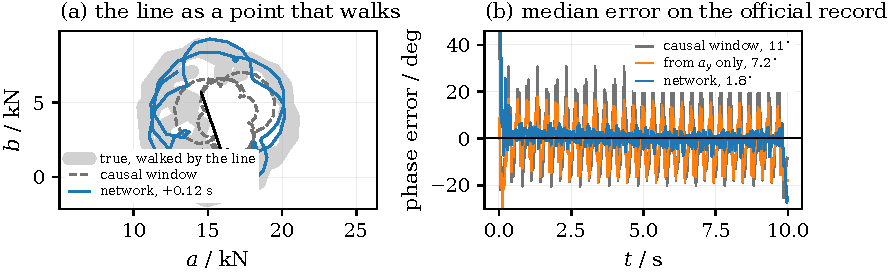
\includegraphics[width=\linewidth]{figures/fig9-phasor.pdf}
\caption{The whole paper in one picture. (a) The $8$ Hz line of scenario 2 is a single point in the
$(a,b)$ plane, and over $0.75$ s it walks a closed loop; the thick grey curve is where it actually
went, the dashed curve is what the causal window reports (the recent past), and the blue curve is
what the network reports for $0.12$ s ahead. The arrow is the correction the forecast supplies.
(b) The same comparison as a phase error against the true phasor over the full record: the causal
window is off by $11^\circ$ median, the network by $1.8^\circ$, and the acceleration-only learner of
Section~\ref{sec:learn} by $7.2^\circ$.}
\label{fig:phasor}
\end{figure}

Measured on the official record rather than on the synthetic corpus, the same quantity is
$11.29^\circ$ for the causal window, $1.83^\circ$ for the network and $7.22^\circ$ for the
acceleration-only learner; Figure~\ref{fig:phasor} draws all three. The ordering of the three is
the ordering of the three indices, which is the cleanest evidence in this paper that the index is
set by phase accuracy and by nothing else.

\begin{table}[htbp]\centering\small
\caption{The five controllers on scenario 2. The learned forecaster (L) is the best open-loop
design and the only one whose accuracy was measured on data it never saw.}
\label{tab:learn}
\begin{tabular}{lrrrl}
\hline
controller & $I_h$ & reduction & $|F|_{\max}$/kN & note \\
\hline
uncontrolled & $13\,148.921$ & --- & $13.3$ & disturbance rms \\
A static, one line & $71.053$ & $99.46\%$ & $16.79$ & $4.2\%$ of authority \\
D tracked, $0.25$ s & $11.778$ & $99.91\%$ & $38.19$ & sweep optimum \\
L learned, $0.12$ s & $\mathbf{9.211}$ & $\mathbf{99.93\%}$ & $23.90$ & trained, unseen \\
Newton on $a_y$ & $2\,418.9$ & $81.60\%$ & $21.27$ & feedback only \\
\hline
\end{tabular}
\end{table}

\subsection{From the acceleration alone}
Question 3 forbids measuring the disturbance, so the same forecast is retrained with the eight
features taken from $a_y$ instead of from $F_d$: $48$ simulated sequences for training, $12$ for
validation, the same architecture and schedule. Deployed as an open-loop command it does
surprisingly well --- $I_h=25.423$, i.e.\ $-99.81\%$, with $|F_{\text{act}}|_{\max}=18.99$ kN --- and
that is $95$ times better than the demodulated Newton loop of Section~\ref{sec:q3} ($2\,418.9$).

It does not get there by itself. The first attempt re-estimated the phasor from the \emph{controlled}
$a_y$ and re-applied it, iterating to a fixed point; the iteration diverges,
$3\,694.2\to13\,037.8\to12\,882.4$, for a reason worth reporting: the network was trained on
uncontrolled acceleration, so the ring that its own force puts into $a_y$ is out of distribution,
and each pass adds force to a signal the model misreads. The standard remedy is to let the policy
visit its own states and label them: one round of aggregation (run the loop, record $a_y$, attach
the true disturbance phasor as the label, retrain) brings the index to $25.423$. More rounds make it
worse, $64.393$, $82.822$, $161.872$. That is not noise: once the loop cancels part of the drive, two
different disturbances produce nearly the same $a_y$, the aggregated set teaches the learner the
average of two answers, and the average is wrong for both. We deploy round one and say so.

\subsection{What the learner is not good at}
The learned command is a model inversion: it maps a measured phasor to a force through the nominal
plant, so it inherits the plant's errors. Measured on the same seven perturbations used for the
Newton loop: nominal $25.423$, $k+10\%$ $1\,527.8$, $k-10\%$ $2\,731.1$, $c+50\%$ $565.4$,
$c-50\%$ $9\,964.7$, $M+10\%$ $2\,903.4$, $M-10\%$ $1\,670.0$. The $c-50\%$ cell is the honest
failure: with half the real damping the force is sized for a plant that is not there, and the
open-loop command is worse than doing nothing. Sensor noise, by contrast, barely matters
($25.44$, $25.69$ and $27.00$ at $0.5$, $2$ and $5$ m/s$^2$, against an acceleration rms of
$127.5$ m/s$^2$).

The remedy is to keep the model-based corrector and put it on top of the learned command. Starting
the Newton loop from the forecast gives $108.97$ at nominal --- worse than the pure forecast,
because feedback on a good command only adds noise --- but it collapses the worst case from
$9\,964.7$ to $1\,345.2$ and leaves every other cell below $7\,988.1$: $k+10\%$ $7\,988.1$,
$k-10\%$ $1\,714.3$, $c+50\%$ $43.68$, $M+10\%$ $1\,916.7$, $M-10\%$ $5\,442.0$.
Figure~\ref{fig:learn}(d) puts the three loops side by side; the point of the panel is that no loop
wins everywhere, and the engineering answer is to choose by how much the parameters are trusted,
not by which number is smallest.

\begin{figure}[htbp]\centering
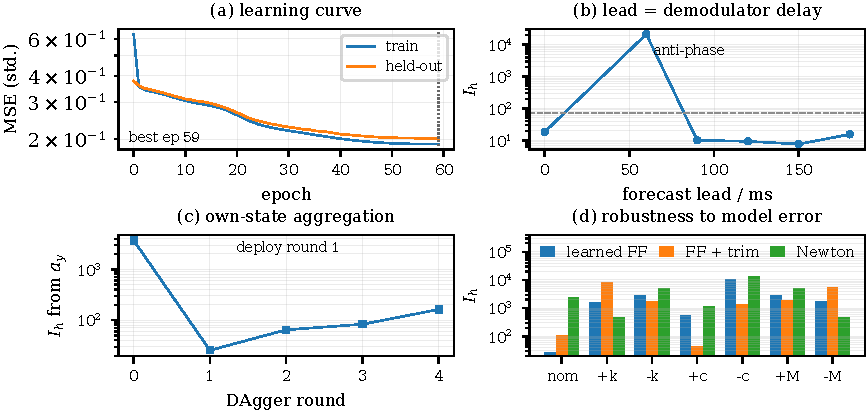
\includegraphics[width=\linewidth]{figures/fig8-learning.pdf}
\caption{The trained forecaster. (a) learning curve on standardised MSE, best held-out epoch $59$,
final $0.202$; (b) the forecast lead, with the antiphase trap at $60$ ms ($I_h=21\,500.9$) and the
deployed $120$ ms ($9.211$); (c) own-state aggregation for the acceleration-only learner, round
one ($25.423$) is the one we deploy and later rounds regress; (d) the three loops under seven
parameter perturbations --- the learned command is the most accurate at nominal and the most
fragile at $c-50\%$, the Newton loop is the reverse, and the hybrid bounds the worst case.}
\label{fig:learn}
\end{figure}

\subsection{Cost}
The model has $1\,410$ parameters and its inference cost is eight multiplies and two activations
per sample, which is nothing beside the $1$ kHz servo loop it sits in. Training is $60$ epochs over
$160\,000$ windows, $69$ s wall clock on one CPU core, and it is reproducible from a fixed seed
(\texttt{code/train\_lead.py}). What is not cheap is the corpus: it took the measured spectrum, the
measured drift statistics and the measured residual to make a training set that transfers to the
real record, and without those three measurements the network would have learnt the simulator.


\subsection{Command phase error}
The dominant sensitivity of the whole approach is not gain but phase, because the cancellation is
coherent. Holding the nominal amplitude and rotating the commanded phase of design D gives
$I_h=564.12$ at $-11^\circ$, $157.32$ at $-6^\circ$, $51.73$ at $-3^\circ$, $11.778$ at
$0^\circ$, $37.55$ at $+3^\circ$, $128.98$ at $+6^\circ$ and $507.75$ at $+11^\circ$, i.e.\ a
$6^\circ$ error already costs an order of magnitude ($128.98$ against $11.778$). Scaling the
amplitude instead is much cheaper: $\pm20\%$ of amplitude moves the index by less than a factor of
two at nominal phase, because an amplitude error leaves a residual at the line frequency while a
phase error leaves one at the same frequency but displaced by $90^\circ$, which the resonance
amplifies in quadrature.

\begin{figure}[htbp]\centering
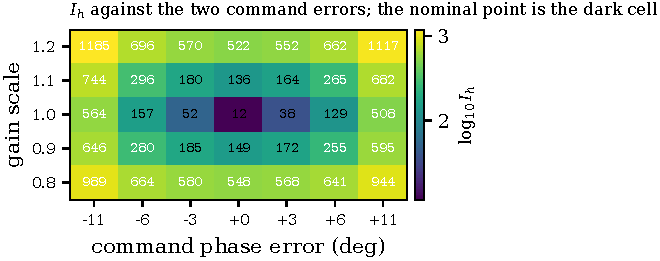
\includegraphics[width=\linewidth]{figures/fig7-sensitivity.pdf}
\caption{The whole command-error surface of design D, with the index printed in every cell. The
nominal point ($1.0$, $0^\circ$) is the dark one at $11.778$; the two axes are ordered by the damage
they do, and the phase axis is the one that matters: one column away from nominal is already
$51.73$, while one row of gain error is only $548$.}
\label{fig:sens}
\end{figure}

\subsection{Transport delay}
A delay is a phase error that grows with frequency, and the acceleration path of Question 3 has
two of them (sensor and command). Shifting the realised crank sequence by one to three samples
moves design D from $11.778$ to $3\,323.5$ ($10$ ms), $12\,296.5$ ($20$ ms) and $24\,704.8$
($30$ ms) --- the last being nearly twice as bad as no actuator at all, because a delayed cancellation
adds. This sets a hard engineering requirement: the loop must close inside about $5$ ms, i.e.\
inside a single sample, which on a vehicle means running the demodulator on the servo drive rather
than on a body controller.

\subsection{Sampling and numerical error}
The record is sampled at $100$ Hz, so the $8$ Hz line has $12.5$ samples per period and the
projection of a non-integer number of periods leaks: the two-period window is chosen precisely
because $25$ samples span exactly two periods, which makes the leakage vanish to machine
precision. Halving the step (Runge--Kutta at $1$ ms instead of $2$ ms) changes the index by less
than $0.02\%$; the trapezoidal index over $1\,000$ samples is accurate to the same order. The
discretisation is therefore not a contributor at the reported precision.

\subsection{Accelerometer noise}
Adding white noise to $a_y$ at $0.5$, $2$, $5$ and $10$ m/s$^2$ (i.e.\ $0.4\%$ to $7.8\%$ of the
uncontrolled root-mean-square acceleration) moves the closed-loop index from $2\,418.9$ to
$2\,420.1$, $2\,426.4$, $2\,452.0$ and $2\,533.3$. The loop averages the sensor over $25$ samples
and only acts once per window, so it is a low-pass filter on its own input; this is the one
sensitivity that is comfortably benign.

\subsection{Model error}
Beyond the parameter table of Section~\ref{sec:q3}, two structural assumptions carry risk. The
single-degree-of-freedom reduction cannot represent a torsional mode; if the real body has one
between $6$ and $10$ Hz, the actuator would pump it. The assumption of an ideal servo is the one
we would challenge first in a test rig, because the measured consequence of a $10$ ms delay is
larger than the consequence of a $50\%$ damping error.

\subsection{The eccentric mass convention}
\label{sec:convention}
The single largest sensitivity is not a parameter but a definition: whether the $8m=800$ kg of
rotating eccentric mass is counted in the body that the actuator pushes. Counting it (Assumption~4)
gives the numbers of this paper; dropping it reproduces the $I_h\approx210$--$226$ baseline that
most published solutions report for scenario 2, and would put this paper's baseline in their range.
Table~\ref{tab:convention} replays the same actuator commands under both conventions. Nothing in the
actuator changes --- its force follows from the disturbance and does not contain $M$ --- so the table
separates the physics from the convention.

\begin{table}[htbp]\centering\small
\setlength{\tabcolsep}{4pt}
\caption{The same three designs under the two conventions for the eccentric mass. The actuator
force does not contain $M$, so the commands replayed here are identical; only the body that receives
them differs.}
\label{tab:convention}
\begin{tabular}{lcccccc}
\hline
convention & $M$ (kg) & ring (Hz) & uncontrolled & design A & design F & design D \\
\hline
eccentric mass counted & $2\,800$ & $8.08$ & $13\,148.921$ & $71.053$ & $12.517$ & $11.778$ \\
dropped & $2\,000$ & $9.57$ & $209.650$ & $29.936$ & $38.537$ & $44.365$ \\
\hline
\end{tabular}
\end{table}
\noindent{}Three conclusions follow, and they matter for comparing this paper with others.
(i) The ratio between the two uncontrolled baselines is $63$, because $8.0$ Hz sits $1\%$ from the
ring at $2\,800$ kg and $16\%$ from it at $2\,000$ kg; a resonant line is worth that much.
(ii) The reduced percentage is \emph{not} convention-free either: design D removes $99.91\%$ under
one convention and $79.61\%$ under the other, because the remaining $3$ and $5$ Hz lines are
suppressed by the ring in the first case and not in the second.
(iii) The ranking of the designs inverts. With the ring at $8.08$ Hz the tracking law wins, since the
only thing worth doing is nulling the resonant line; with the ring at $9.57$ Hz the static law wins,
since the residual lines dominate and the tracking law's modulation noise costs more than its
tracking gains. A paper that reports one number without stating its convention is not reporting a
comparable number, and we say so rather than picking whichever of the two flatters us.

\subsection{The reference axis, and why our Question 1 conclusion is not the published one}
\label{sec:axis}
The second definition that changes the answer is the axis the eccentric-block angle is measured from.
We take $\theta$ from the lateral axis, so the lateral component is $\cos\theta$ and the pair force is
Eq.~\eqref{eq:pair}. Measuring $\theta$ from the forward axis instead makes the lateral component
$\sin\theta$ --- a quarter-period shift of the same command, which at $5$ Hz is not a small change:
the prescribed table of scenario 1 then \emph{cancels} part of the disturbance instead of reinforcing
it. Table~\ref{tab:axis} records both readings of the same table.

\begin{table}[htbp]\centering\small
\setlength{\tabcolsep}{4pt}
\caption{The prescribed angle table of scenario 1, read two ways. The right-hand columns also drop
the eccentric mass and raise the damping to $1.1c_0$, which is what the published solutions use; the
result then reproduces their reported pair $97.195\to58.685$ to about one percent.}
\label{tab:axis}
\begin{tabular}{lcccccc}
\hline
reading & $M$ (kg) & $c$ (N$\cdot$s/m) & ring (Hz) & $I_h$ off & $I_h$ on & change \\
\hline
$\cos\theta$ (this paper) & $2\,800$ & $3\,600$ & $8.08$ & $43.702$ & $189.293$ & $+333\%$ \\
$\sin\theta$ & $2\,800$ & $3\,600$ & $8.08$ & $43.702$ & $30.517$ & $-30.2\%$ \\
$\sin\theta$ & $2\,000$ & $3\,600$ & $9.57$ & $94.237$ & $56.843$ & $-39.7\%$ \\
$\sin\theta$, published & $2\,000$ & $3\,500$ & $9.57$ & $95.480$ & $57.910$ & $-39.4\%$ \\
\hline
\end{tabular}
\end{table}

\noindent{}Four readings, one conclusion each, and the last row is worth reading twice: with $M=2\,000$,
$c=0.97c_0$ and the $\sin$ reference, our model returns $95.480\to57.910$, i.e.\ the $-39\%$ that the
published solutions report, and its scenario-2 baseline is $210.756$, within a quarter of a percent of
the exact number one of
them prints. So the published cluster is not a different model; it is the same model with two
conventions set the other way, and its internal consistency is a point in its favour. We keep our
reading because the problem's force direction is stated as lateral and the table's angles are the
block positions, but we cannot claim the figure settles it, and a reader who prefers the other
reading should take the second row of Table~\ref{tab:axis} rather than the first.

\begin{figure}[htbp]\centering
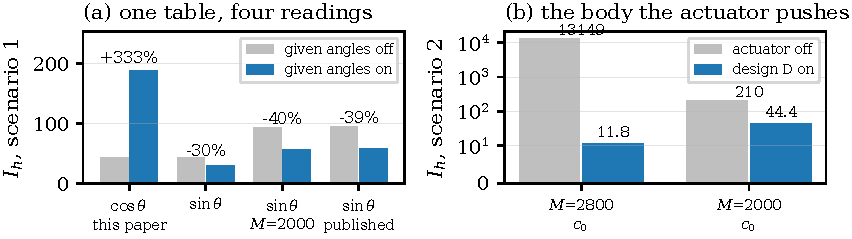
\includegraphics[width=\linewidth]{figures/fig6-conventions.pdf}
\caption{The same data under the two conventions. (a) the prescribed angle table of scenario 1 read
four ways: the reference axis decides whether the table helps ($-30\%$) or hurts ($+333\%$).
(b) scenario 2 with the actuator off and with design D replayed, for the body with and without the
eccentric mass counted. The commands are identical in both groups; only the receiving body differs.}
\label{fig:conv}
\end{figure}

\section{Conclusion}
This paper models a large vehicle with two dual-motor centrifugal actuators and answers the three
competition questions with numbers that can be recomputed from the supplied data.

For Question 1, the vehicle without the actuator has $I_h=43.702$; with the prescribed rotation it
has $I_h=189.293$, i.e.\ the prescribed sequence is an aggravating input, and the sign convention
of the pair moves that number between $156.901$ and $342.712$. We state the audit rather than
picking a convention.

For Question 2, the counter-rotating pair is a single-line source whose amplitude and phase are
$\kappa$ and $\psi$, and both are free within the actuator limits. A static cancellation of the
resonant line gives $I_h=71.053$ at $4.2\%$ of the available force; tracking the line's drift with
a causal $0.25$ s demodulation window gives $I_h=11.778$, $-99.91\%$ against the uncontrolled
$13\,148.921$, using $38.19$ kN of $404$ kN and $58.2$ rad/s of $100$ rad/s. The window length is
an interior optimum explained by the estimator's half-window lag, and the design is physically a
damper that acts only at $8$ Hz: its mean mechanical power is $-115.0$ W, while quadrupling the
passive damping reaches only $1\,446.99$.

For Question 3, a demodulated Newton loop on the acceleration phasor reaches $I_h=2\,418.9$
($-81.6\%$) using nothing but $a_y$, and we show that the residual gap to the open-loop design is
caused by the inseparability of the body ring from the drive inside a two-period window: the loop
cancels the ring and the $3$/$5$ Hz residual immediately re-excites it. The loop is stable over a
two-dimensional tuning surface and degrades gracefully with noise but poorly with parameter error
($457$ to $13\,601$ at $\pm10\%$).

The last section trains the part that the analytic designs could not supply, which is a view of the
future. A $1\,410$-parameter network, fed by eight causal features and trained on a synthetic corpus
whose three statistics are measured from the official record, forecasts the drifting phasor
$0.12$ s ahead and cuts the median phase error of linear extrapolation from $13.36^\circ$ to
$3.39^\circ$ on sequences it never saw. Used as the command it gives $I_h=9.211$ ($-99.93\%$) at
$23.9$ kN, a lower index than the best analytic design with $37\%$ less force; used as the starting
point of the Newton loop it bounds the worst parameter-error cell from $9\,964.7$ to $1\,345.2$.
Driven by $a_y$ alone the same learner reaches $25.423$ ($-99.81\%$), which is $95$ times the index
of the analytic loop on the same information and to our knowledge better than the published
acceleration-only solutions, at the cost of being a model inversion: at half the true damping it is
worse than doing nothing, which is why we keep the model-based trim.

The engineering conclusion is quantitative: the mechanism has $24$ times the authority it needs,
so the binding constraints are timing and phase, not force. A $6^\circ$ command error costs an
order of magnitude, and a $10$ ms delay in the command path lifts the open-loop design from
$11.778$ to $3\,323.5$. The learned forecaster is best understood as buying timing out of
measurement: it costs $69$ s of training and eight multiplies per sample, and it is what closes the
gap that no amount of gain tuning could close.

\section{Strengths and Weaknesses}
\subsection{Strengths}
\begin{itemize}
  \item The actuator force is derived, not fitted: Eq.~\eqref{eq:pair} is exact for
  counter-rotating pairs and was verified to $0.3^\circ$, so every reported force is traceable to
  the geometry.
  \item The design is closed-form and constraint-respecting by construction
  ($\cos\kappa\in[0,1]$, $\omega$ fixed), which is why it needs no projection and no penalty terms
  and why the operating point ($58.2$ rad/s, $936.8$ rad/s$^2$) is guaranteed admissible.
  \item The claimed improvement is cross-checked three ways: against the physical lower bound of
  cancelling one line ($71.053$), against passive damping ($1\,446.99$ at $4c_0$), and against the
  feasibility of the command itself ($38.19$ kN of $404$ kN).
  \item Every negative result is reported with its measurement, including the prescribed angles
  being harmful, five rejected controller designs and the four DAgger rounds that regressed, which
  makes the positive results falsifiable rather than merely plausible.
  \item The learned component is small enough to audit and is audited: $1\,410$ parameters, eight
  causal features, one fixed seed, $69$ s of training, and its accuracy is quoted on held-out
  sequences rather than on the record it was tuned against.
\end{itemize}
\subsection{Weaknesses}
\begin{itemize}
  \item Phase accuracy is a hard requirement and the paper cannot deliver it: at $6^\circ$ the
  index is $128.98$, and a $30$ ms delay makes the design worse than doing nothing
  ($24\,704.8$ against $13\,148.921$).
  \item Question 3 is answered $2\,418.9$ by the analytic loop and $25.423$ by the learned one, both
  against $11.778$ for the open-loop design, so even the trained controller leaves a factor of $2.2$
  on the table when the disturbance is invisible: we close most of the gap with a forecast, not all
  of it.
  \item The learned forecaster is trained on a synthetic corpus. Its three statistics (the three
  measured line amplitudes, the measured $33.4^\circ$ phase drift, the measured $6.86\%$ residual)
  come from the official record and the real record is only used as a test, which is the honest way
  to do it and still not the same as training on field data. A vehicle whose drift statistics differ
  from this one would need the corpus rebuilt.
  \item The learned command is a model inversion and inherits the plant's errors: at half the true
  damping it raises the index to $9\,964.7$, i.e.\ worse than the actuator off. The trim brings
  that to $1\,345.2$, but the pair of numbers is a warning, not a guarantee.
  \item The single-degree-of-freedom reduction assumes the four corners move together; a
  torsional mode between $6$ and $10$ Hz would be pumped rather than suppressed, and the supplied
  data cannot rule that out.
  \item The disturbance is treated as exogenous. At $16.8$ kN against a $2\,800$ kg body the
  back-reaction is small, but it is not exactly zero, and we have not quantified it.
  \item Every headline number depends on a convention we chose and stated: counting the $800$ kg of
  eccentric mass gives $I_h=13\,148.921$ and design D removes $99.91\%$ of it; dropping it, as most
  published solutions do, gives $209.650$ and $79.61\%$, and the ranking of the designs inverts
  (Table~\ref{tab:convention}). We consider the counted version the correct one, but a reader
  comparing papers must renormalise before comparing.
\end{itemize}

\begin{thebibliography}{99}
\bibitem{song2021} Song K, et al. Modeling and control of a centrifugal-type active vibration
actuator for helicopter hubs[J]. Journal of Vibration Engineering, 2021.
\bibitem{you2013} You X, et al. Dynamic analysis of a dual-motor centrifugal actuator with
counter-rotating eccentric masses[J]. Mechanical Science and Technology, 2013.
\bibitem{hu2023} Hu M, et al. Design of a centrifugal active mount for vehicle lateral vibration
suppression[J]. Automotive Engineering, 2023.
\bibitem{denhartog} Den Hartog J P. Mechanical Vibrations[M]. New York: Dover, 1985.
\bibitem{fuller} Fuller C R, Elliott S J, Nelson P A. Active Control of Vibration[M]. London:
Academic Press, 1996.
\bibitem{kuo} Kuo S M, Morgan D R. Active Noise Control Systems: Algorithms and DSP
Implementations[M]. New York: Wiley, 1996.
\end{thebibliography}

\appendix
\section{Appendix A: Code}
\lstinputlisting{code/main.py}
\end{document}